
\documentclass[12pt]{article}
\usepackage[utf8]{ inputenc}
\usepackage[brazil]{babel}
\usepackage{hyperref}
\usepackage{graphicx}
\usepackage{geometry}
\geometry{left=2.5cm,right=2.5cm,top=2.5cm,bottom=2.5cm}

\graphicspath{{../../imagens/}}
\hypersetup{
    colorlinks=true,
    linkcolor=blue,
    filecolor=magenta,
    urlcolor=cyan,
}
\title{\textbf{LDO - Capítulo 3\\
Como é feito esse aprendizado de máquina}}

\author{Homenique}
\date{23/10/2020}

\begin{document}
    \maketitle

        Quando vamos falar de Machine learning, é importante entendermos como as máquinas aprendem. de forma bem simples podemos dividir em 3 grupos de formas de aprendizados 
        \begin{itemize}
            \item Aprendizado Supervisionado
            \item Aprendizado Não supervisionado
            \item Aprendizado Por reforço
          \end{itemize}
          vamos conhecer um pouco de cada um?
    
            %texto 1
            \begin{figure}[ht]
                \centering
                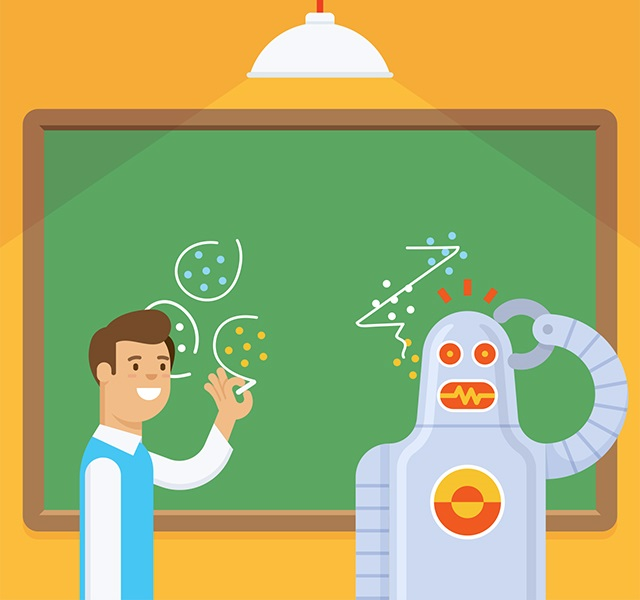
\includegraphics[scale=0.5]{robo_aprendedo.jpg}               
            \end{figure}
            
            \clearpage
            
            \section{Aprendizado Supervisionado:}

                \paragraph{}Aprendizagem supervisionada é a tarefa de encontrar uma função a partir de dados de treinamento rotulados. O objetivo é encontrar os parâmetros ótimos que ajustem um modelo que possa prever rótulos desconhecidos em outros objetos (o conjunto de teste). Se o rótulo é um número real, a tarefa chama-se regressão. Se o rótulo vem de um conjunto finito e não ordenado, então a tarefa chama-se classificação.

            %texto 2 
           \section{Não supervisionado:}
                \paragraph{}Na aprendizagem não-supervisionada temos menos informação sobre os objetos, em particular, o conjunto de treinamento não é rotulado. O nosso objetivo, neste contexto, é observar algumas similaridades entre os objetos e incluí-los em grupos apropriados. 
                
                \begin{figure}[ht]
                    \centering
                    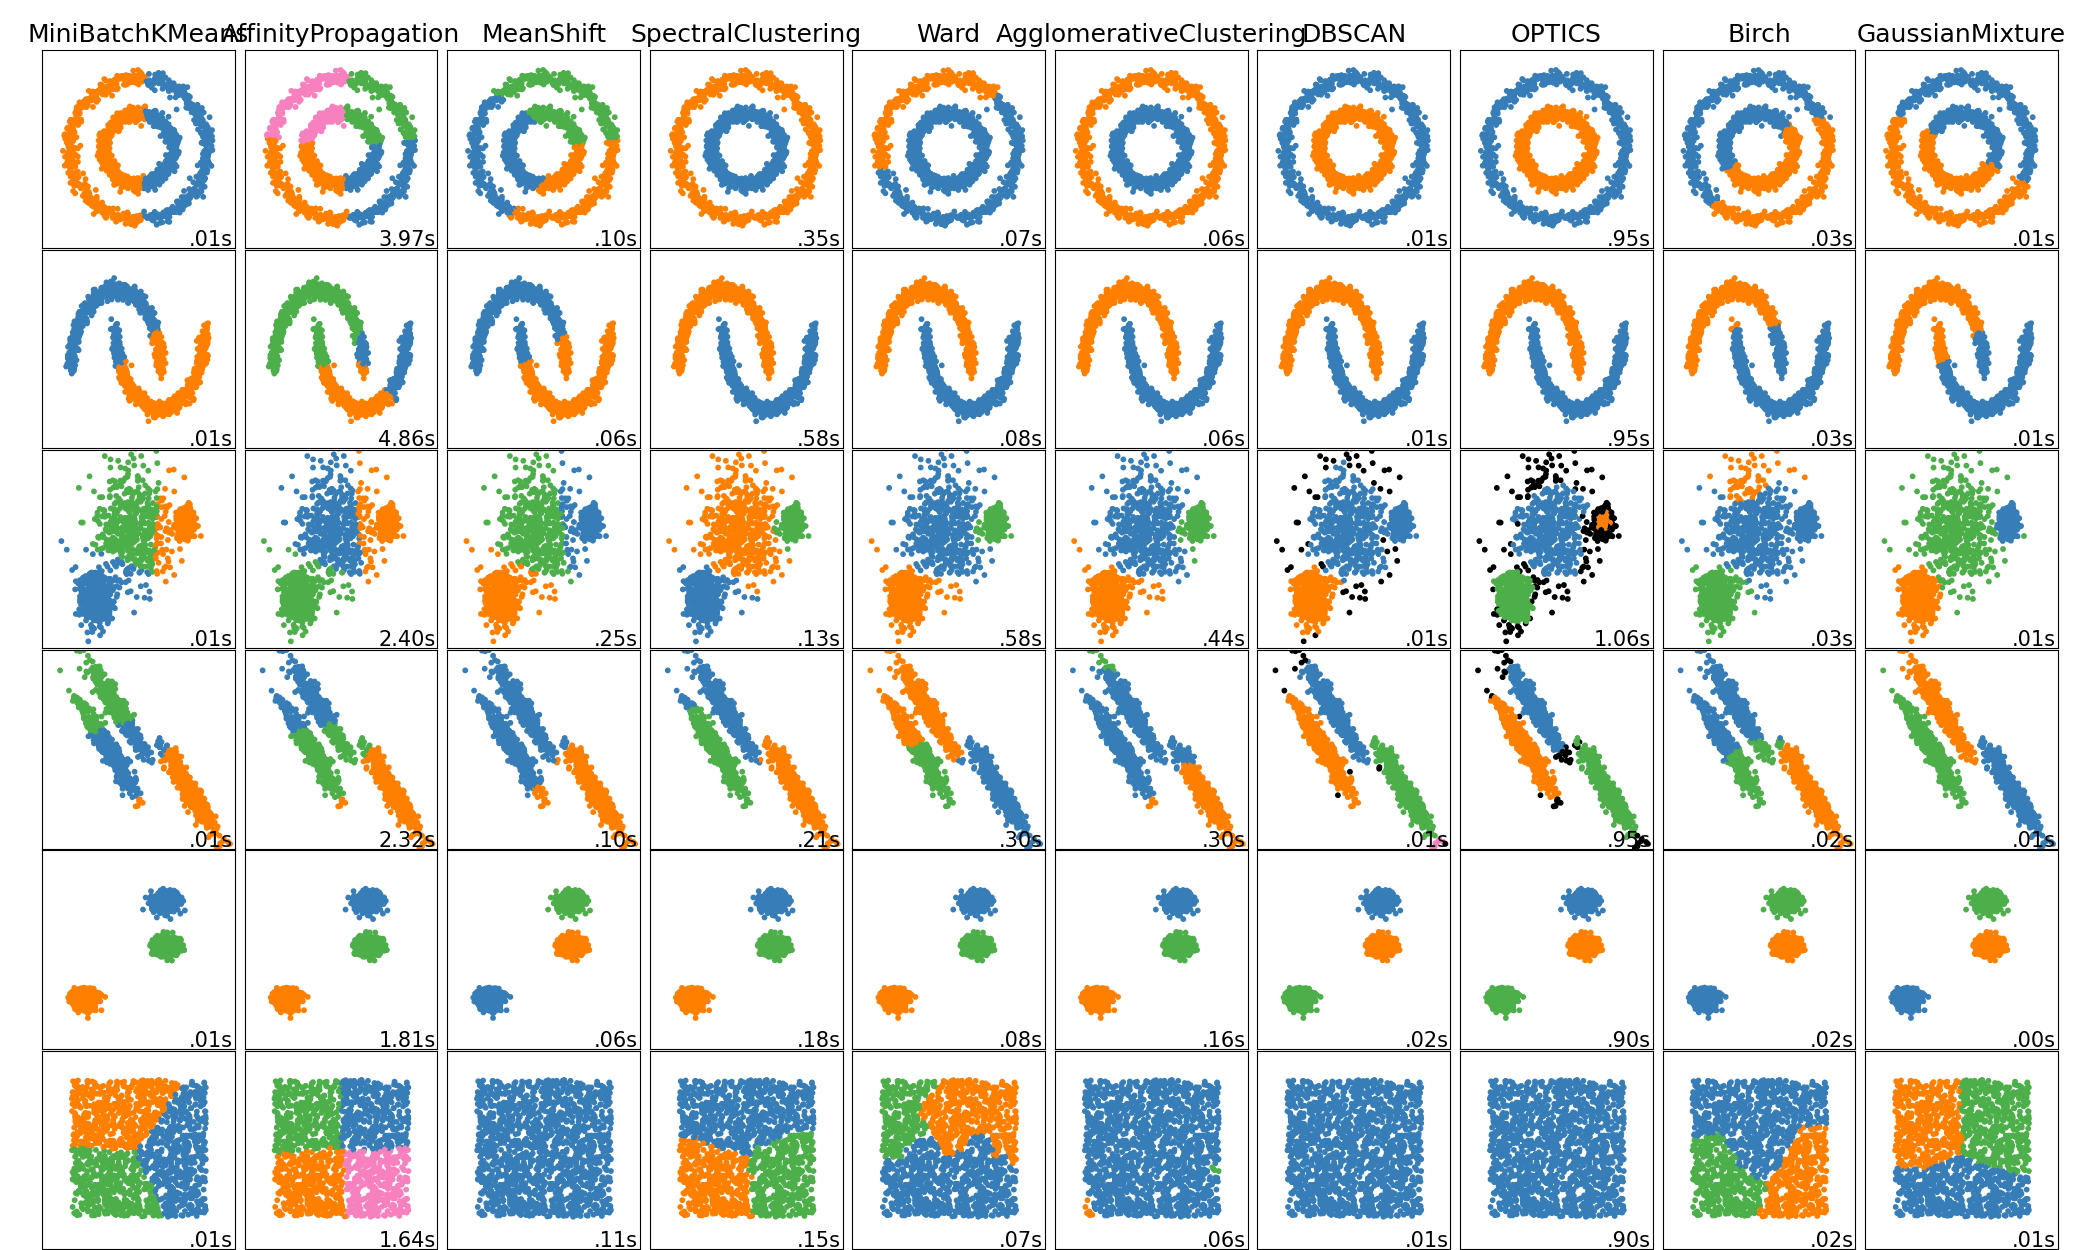
\includegraphics[scale=0.3]{classificação de grupos.png}               
                \end{figure}
                        Alguns objetos podem diferir largamente de todos os grupos e, deste modo, podemos assumir que estes objetos são anomalias.
           
            %texto 3
            \clearpage
           \section{Por reforço:}
                \begin{figure}[ht]
                    \centering
                    
\includegraphics[scale=0.2]{jack-jack-num-num-cookie_orig.png}
                \end{figure}
   
                \paragraph{}Aprendizagem por reforço é uma área de aprendizagem de máquina que investiga como agentes de software devem agir em determinados ambientes de modo a maximizar alguma noção de recompensa cumulativa.
         

  
\end{document}